\chapter{\sf Introduction}\label{ch:intro}

The fields of materials science and engineering are built on a solid understanding of phase transitions, which dictate the microstructure, and hence properties, of most man-made materials.
As the rapid pace of technological progress requires materials with ever more demanding specifications, ranging from stronger steels for taller skyscrapers to semiconductors with finely tuned electronic band structures, constant pressure is placed on these fields to enhance their phase transition models and apply them to the development of novel materials.
The advent of plentiful and inexpensive computing power in the past few decades has greatly benefited this endeavor by allowing the numerical study of phase transition problems that prove intractable otherwise.



In particular, great effort goes into the numerical modeling of polycrystalline materials, which are comprised of numerous microscopic interlocked crystal grains (aka. crystallites) of differing sizes, shapes, orientations, and compositions. These materials include most metals and alloys, as well as some ceramics and polymers, and even a few biological microstructures \cite{jin03}. The morphological and chemical properties of the constituent crystal grains have a direct effect on characteristics of the macroscopic material \cite{granasy_phasefieldnuc,boettinger00}, hence the interest in modeling their formation and evolution. The first step in the grains' formation is the process of nucleation, wherein thermal fluctuations in a progenitor phase stochastically create stable nuclei of a new phase which then proceed to grow. The main difficulty in modeling this process is due to the large range of scales involved: though final grains range in size from a few nanometers to above millimeters depending on the material, the initial nuclei form on atomic lengthscales. Further, some systems are known to exhibit nucleation events simultaneously with large-scale structure evolution, such as in rapidly cooling metal pools formed by laser-beam welding \cite{david03,boettinger00}, and during the so-called columnar to equiaxed transition \cite{kurz01}. While the growth and late evolution of grains are relatively well understood \cite{granasy_02}, there remain open questions concerning how to efficiently and accurately model the initial nucleation stage of formation without impairing the modeling of the much larger scale evolution. 

Various numerical techniques for simulating phase transition processes, including nucleation, have been developed since the 1960s, each best suited to specific types of problems. Among these, traditional phase field methods \cites{hohenberg77,singer08,chaikin_condensed,provatas_PFC} are some of the more widely used in studying microstructure formation. They are well-adapted for simulations on micrometer to millimeter length scales, and on diffusive time scales. These methods consist of multi-field descriptions of phases separated by diffuse interfaces, effectively greatly refined versions of Landau's order parameter theory of phase transition. The fields are spatially continuous, constant within bulk regions, and vary smoothly but rapidly at interfaces. Typically, the fields used can represent order, concentration, and temperature. Phase field methods have been used to simulate assorted material phenomena that include eutectic (multi-species solid mixture) system growth \cite{grant94}, dendritic microstructure evolution \cite{provatas98,kim99}, fracture growth \cite{karma01}, and structure changes in irradiated materials \cite{li17}. However, they face difficulty in modeling physical processes that involve atomistic lengthscales. For example, phenomena that occur on the scale of the width of phase interfaces need special care \cite{karma01_2,elder01,plapp11}, as the phase field models approximate interfaces to be much more diffuse than the typical dozen atom-widths found in real materials, for reasons of computational efficiency. Moreover, effects related to crystalline lattice structure, such as orientation and elastic deformation, do not appear naturally in the basic models, instead requiring more coupled fields to be added \cite{oforiopoku2010,steinbach06,granasy_phasefieldnuc,plapp11} and thus increasing computational and mathematical complexity. As nucleation is a fundamentally atomistic process, phase field models are incapable of modeling it exactly: the processes leading to formation of physically-accurate nuclei can not be resolved at these models' scales. Workarounds to this limitation involve either using unrealistically large thermal fluctuations that force nucleation at the desired time and length scales, or artificially adding already-formed nuclei to the system according to assumed statistics for the material \cite{granasy_phasefieldnuc,granasy_02,plapp11}.

On the other end of the scale spectrum for modeling techniques, atomistic models, such as the Molecular Dynamics (MD) methods \cite{alder59,rapaport_md}, are capable of simulating phenomena difficult to access with phase field methods. These include amorphous solidification of metals \cite{ozgen04,tian08}, properties of atomically-rough interfaces \cite{hoyt01}, and more. Notably, MD methods have had recent success in simulating nucleation and nanoscale grain growth in metals \cite{shibuta15}. These methods typically involve tracking the individual positions and interaction potentials of all the atoms in a system, calculating the dynamics of the resulting N-body problem by numerical integration of Newton's equations of motion. However, the large number of atoms tracked by these methods limits the length and time scales that can reasonably be simulated with current computational speeds to nanometers and nanoseconds respectively. This prevents the scaling of atomistic models for the study of mesoscale structure dynamics, including those that would result from or occur concurrently with nucleation-initiated phase transitions.

Recently, the Phase Field Crystal (PFC) model as first proposed by Elder et al. \cites{elder02,provatas07,emmerich12,humadi13,provatas_PFC} has emerged as a modified phase field method that aims to bridge the gap between atomistic models such as MD and mesoscale models such as traditional phase field methods. Similar to traditional phase field models, the PFC model represents material with a continuous spatial field. However, this field is now periodic in bulk regions, instead of constant. The periodic field acts as an atomic density field, with its peaks denoting the most likely position of the crystal lattice's atoms. Its amplitude represents a phase's order, with the field having zero amplitude in liquid phases and nonzero in solid phases. Figure \ref{fig:phasefield_profile} sketches the profiles of the phase fields in traditional phase field models and the PFC model at a solid-liquid interface, for comparison. In contrast to traditional phase field methods, the PFC method does not have difficulty in describing aspects of the crystal lattice structure, including different grain orientations, grain boundary dynamics \cite{elder08}, lattice defects, and elastoplasticity \cite{elder02,humadi13}. Figure \ref{fig:pfc_example} shows the result of a PFC simulation of solidification for a two-dimensional solid with triangular lattice structure, including some defects that arise in the crystal lattice.

Unlike in `true' atomistic models, atomic movement on vibrational timescales in the PFC model is effectively averaged out, leaving only movement on diffusive timescales. It has been shown \cite{grant08} that applying coarse-graining in time on atomistic simulation methods such as MD methods recovers similar results as the PFC model. Compared to MD methods, PFC is computationally more efficient due to the lack of tracking of individual atoms. This allows studying phenomena appearing at longer time and length scales than MD is reasonably able to simulate \cite{dantzig12}.

\begin{figure}[h]
\centering
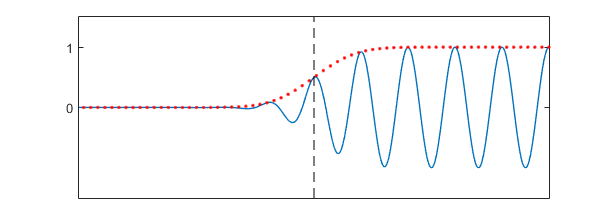
\includegraphics[width=1\textwidth]{fig_pfc/phasefield_profile.png}
\caption{Sketch of profile of phase fields in traditional phase field models (red) and in the PFC model (blue). The x-axis is one dimension of space, and the y-axis is value of the phase field. The vertical dashed line denotes the position of a solid-liquid interface, with the liquid bulk on the left and the solid bulk on the right.}\label{fig:phasefield_profile}
\end{figure}

\begin{figure}[!ht]
\centering
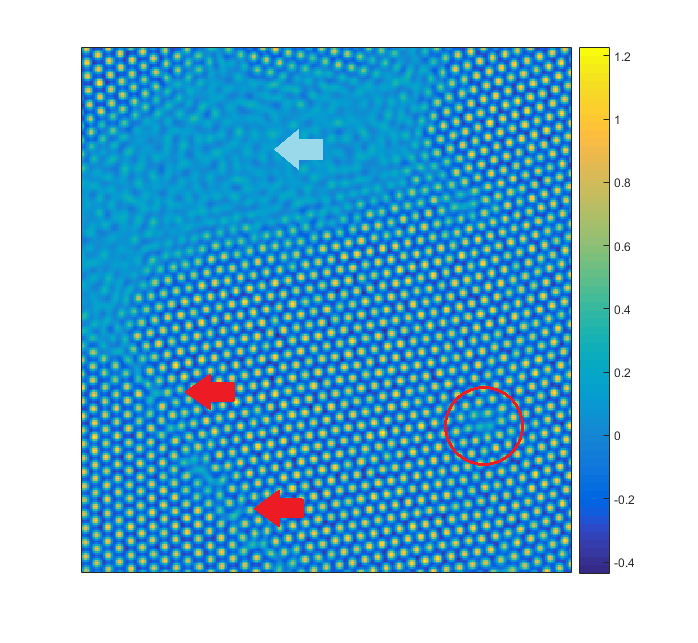
\includegraphics[width=1\textwidth]{fig_pfc/pfc_example_mod2.png}
\caption{Results of a PFC simulation for solidification, showing the phase field in adjacent solid regions with triangular lattices of different orientations, in coexistence with a liquid region. The cyan arrow points to the region of fluctuating liquid, between solid regions. The red arrows point towards a grain boundary between two solid regions of differing orientations. The red circle shows an isolated dislocation defect.}\label{fig:pfc_example}
\end{figure}

For the reasons stated above, the PFC model can be used as an intermediate model between atomistic simulations and the more coarse-grained traditional phase field methods that do not retain the details of the atomic structure. It is thus of interest to examine whether this model can be used to study the process of nucleation without a loss of efficiency nor accuracy. Nucleation is known to occur naturally in the PFC model through the inclusion of thermal fluctuations obeying the fluctuation-dissipation theorem, with the resulting nuclei consisting of few `atoms' as would be expected in a physical system. More specifically, Granasy, Tegze, Toth, and Pusztai have studied aspects of nucleation in the PFC model including nucleation energy barriers, possible amorphous precursor phases, and heteroepitaxy \cite{toth10,toth11}. However, it is yet unclear whether the PFC model can reproduce specifics of the nucleation process predicted by classical nucleation theory, such as the scaling of nucleation rate and incubation time with temperature. The purpose of this thesis is to numerically study the rates of nucleation in the most basic two-dimensional version of the PFC model, for different parameter choices. We aim to compare these rates to those predicted by classical nucleation theory. We also examine the form of stable nuclei in PFC model simulations, as well as their early-time behavior.

The remainder of the thesis is structured as follows. In chapter \ref{ch:pfc}, following a somewhat more detailed description of general phase field models, the PFC model is introduced and its equilibrium and dynamic properties are examined. Chapter \ref{ch:nucleation} introduces the fundamental concepts of classical nucleation theory. The implementation of the numerical tools used to study the material of the previous two chapters is given in chapter \ref{ch:numerics}. Finally, chapter \ref{ch:results} presents a few results of our investigation on nucleation in the PFC model, followed by our concluding summary and thoughts in chapter \ref{ch:conclusion}.

\textit{Note to the reader: All chapter, section, equation, and figure references, as well as citations, are hyperlinked in the digital PDF version of this work, for convenience.}



